\chapter{Getting Started}\label{ch:GettingStarted}
\section{Installation von Python und VSCodium}
Um mit dem Programmieren loslegen zu können, müssen wir zuerst die Programmiersprache auf unserem Computer installieren, sowie einen guten Code-Editor, mit welchem wir Python-Code schreiben und ausführen können. Ein solches Programm wird typischerweise \gls{IDE} genannt. In diesem Skript verwenden wir die kostenfreie Programmiersprache \textit{Python}, sowie die ebenfalls kostenfreie, weit verbreitete \gls{IDE} mit dem Namen \textit{VSCodium}. Der nachfolgende Abschnitt leitet Sie durch die Installation sowohl auf Windows wie auf MacOS.

\subsection{Anleitung für MacOS}
Um VSCodium unter MacOS zu installieren, benötigen Sie zuerst den Paket-Manager \texttt{brew}. Was macht \texttt{brew}? Laut der \href{https://brew.sh/de/}{offiziellen Webseite}: \enquote{Homebrew installiert Zeug, das du brauchst, das Apple aber nicht mitliefert.}

Falls Sie \texttt{brew} noch nicht auf Ihrem Mac installiert haben, tun Sie dies wie folgt:
\begin{enumerate}
	\item Öffnen Sie ein neues Terminal-Fenster, indem Sie zunächst die Spotlight-Suche mit \keys{\cmd+\space} (\keys{\cmd} +  Leertaste) öffnen. In der Spotlight-Suche müssen Sie nun den Suchbegriff \texttt{Terminal} eingeben und schliesslich die Suchanfrage mit Drücken der Taste \keys{\return} (\texttt{ENTER}-Taste) ausführen.
	\item Geben Sie folgende Code-Zeile ein und führen Sie diese aus (indem Sie mit der \keys{\return}-Taste bestätigen):
	      \begin{lstlisting}[language=bash, numbers=none]
            /bin/bash -c "$(curl -fsSL https://raw.githubusercontent.com/Homebrew/install/HEAD/install.sh)"
        \end{lstlisting}
\end{enumerate}

Führen Sie danach folgende Befehle einzeln aus (jeweils durch das Drücken der \keys{\return}-Taste), um VSCodium und Python zu installieren:
\begin{lstlisting}[language=bash, numbers=none]
brew install --cask vscodium
\end{lstlisting}
\begin{lstlisting}[language=bash, numbers=none]
brew install python3
\end{lstlisting}

Nun sollten sowohl VSCodium als auch Python installiert sein. Falls Sie VSCodium nicht öffnen können und stattdessen eine Sicherheits-Warnmeldung erhalten, folgen Sie \href{https://support.apple.com/de-ch/guide/mac-help/mh40616/mac}{dieser Anleitung}, um das Programm dennoch zu öffnen.

\subsection{Anleitung für Windows}
Öffnen Sie das Programm \texttt{PowerShell} (Sie können mit dem \keys{\faWindows}-Taste danach suchen) als \textbf{Administrator}. Bei uns sieht die Situation aus wie in \cref{fig:PowerShell}.
\begin{figure}[H]
	\centering
	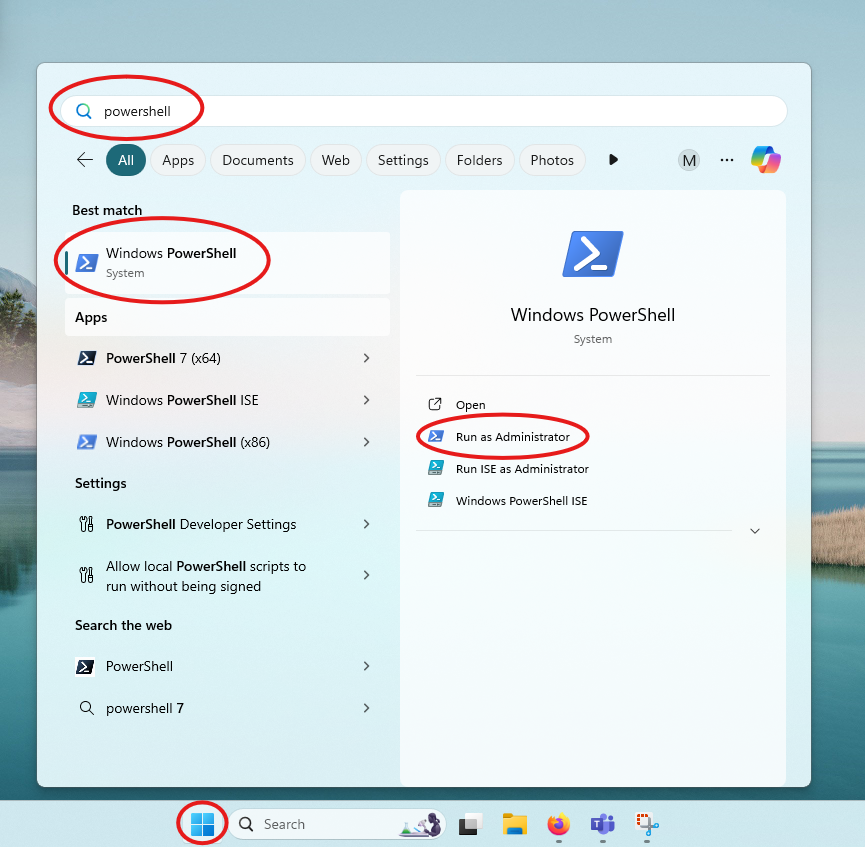
\includegraphics[width=0.6\textwidth]{GrundlagenInfo/00_Programmieren/Skript/Figures/PowerShell.png}
	\caption{\texttt{PowerShell} unter Windows als \textbf{Administrator} öffnen.}
	\label{fig:PowerShell}
\end{figure}

In der \texttt{PowerShell} geben Sie folgende Zeile ein, um den Package-Manager \texttt{winget} zu installieren (bestätigen mit der \keys{\return}-Taste):
\begin{lstlisting}[language=bash, numbers=none]
    winget install -e --id Microsoft.PowerShell
\end{lstlisting}

Führen Sie danach folgende Befehle einzeln aus (jeweils durch das Drücken der \keys{\return}-Taste), um VSCodium und Python zu installieren:
\begin{lstlisting}[language=bash, numbers=none]
    winget install -e --id VSCodium.VSCodium
\end{lstlisting}

Der folgende Befehl listet die verfügbaren Python-Versionen auf. Führen Sie ihn aus und merken Sie sich die höchste Versionsnummer (so ist zum Beispiel Python 3.12 > Python 3.11):
\begin{lstlisting}[language=bash, numbers=none]
    winget search --id Python.Python
\end{lstlisting}
Installieren Sie nun die neuest (höchste Nummer) Version von Python mit dem nachfolgenden Befehl. \textcolor{Fuchsia}{Dabei muss allerdings der Platzhalter \texttt{.3.\_\_} durch die neueste Versionsnummer von Python ersetzten (e.g. anstelle von \texttt{.3.\_\_} muss \texttt{.3.12} stehen).}
\begin{lstlisting}[language=bash, numbers=none]
    winget install -e --id Python.Python.3.__ --scope machine
\end{lstlisting}

Sie können nun mit der \keys{\faWindows}-Taste das Programm-Menu öffnen und nach \textit{VSCodium} suchen, welches nun installiert sein sollte.

\section{VSCodium für Python konfigurieren (MacOS und Windows)}
Im Folgenden müssen Sie Pop-Ups der Form wie sie in \cref{fig:TrustAuthor} gezeigt sind, stets mit \texttt{Yes, I trust the authors} bestätigen.
\begin{figure}[H]
	\centering
	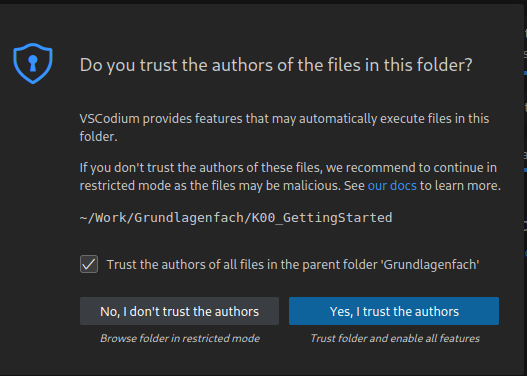
\includegraphics[width=0.5\textwidth]{GrundlagenInfo/00_Programmieren/Skript/Figures/Trust_Authors.png}
	\caption{Meldungen dieser Art können Sie mit \enquote{Ja / Yes} bestätigen.}
	\label{fig:TrustAuthor}
\end{figure}
Öffnen Sie zunächst VSCodium und betrachten Sie \cref{fig:PythonExtension}. Navigieren Sie mit der Maus ganz links zu den \textit{Extentions} (Baustein-Icon) und suchen Sie im Suchfeld nach \textit{python}. Installieren Sie die Erweiterung gemäss \cref{fig:PythonExtension}\footnote{Python language support with extension access points for IntelliSense (Pylance), Debugging (Python Debugger), linting, formatting, refactoring, unit tests, and more.}
\begin{figure}[H]
	\centering
	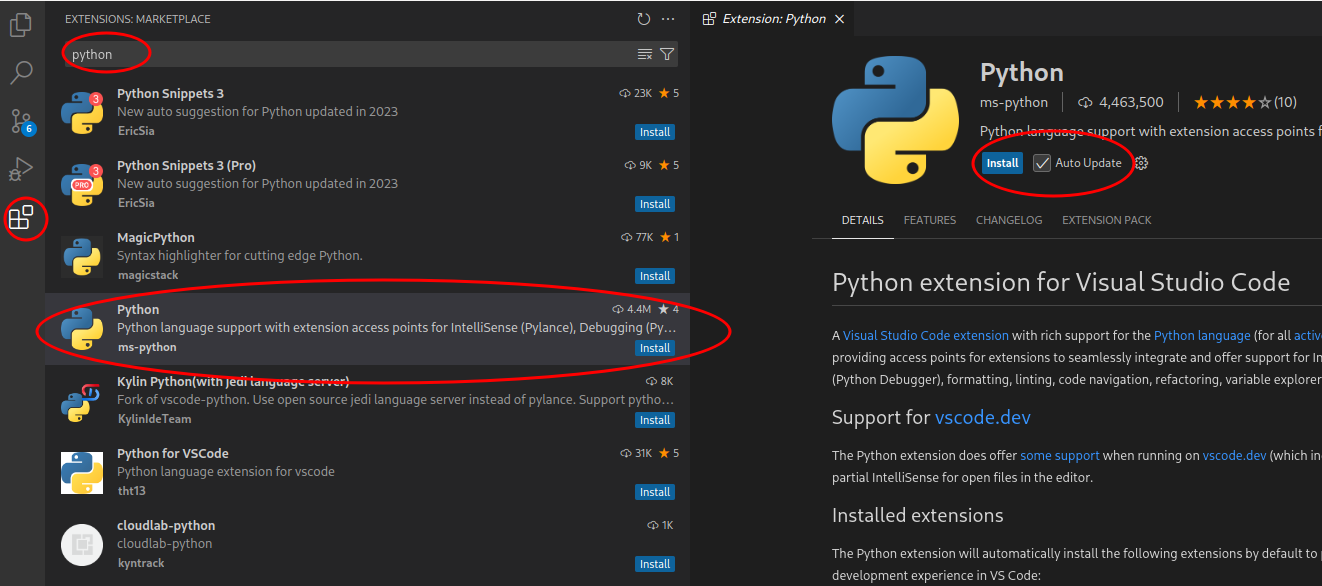
\includegraphics[width=0.9\textwidth]{GrundlagenInfo/00_Programmieren/Skript/Figures/Python_Language_Support_Extension.png}
	\caption{Installation der Python-Extension in VSCodium.}
	\label{fig:PythonExtension}
\end{figure}

\section{Ordner / Verzeichnis für meine Programme}
Wir empfehlen Ihnen, einen neuen Ordner (ein neues Verzeichnis) zu erstellen. Darin sollten Sie in Zukunft alle Programme, welche Sie im Grundlagenfach Informatik schreiben, abspeichern und verwalten. Wir haben das entsprechende Verzeichnis deshalb einfach ``\texttt{Grundlagenfach}'' genannt. Am besten erstellen Sie Ihren Ordner in einem \textbf{Cloud-Service}, den Sie verwenden (z.B. \texttt{OneDrive}). Dadurch werden Ihre Daten zwischen all Ihren Geräten synchronisiert. In diesem Ordner sollten Sie keine persönlichen Daten ablegen.

Nun sind wir bereit, unser erstes Python-Programm zu schreiben und auszuführen.

\begin{enumerate}
	\item In VSCodium, klicken Sie \texttt{File} und dann \texttt{Open Folder...} und navigieren Sie zu dem Ordner, den Sie erstellt haben.
	\item Erstellen Sie in diesem Ordner ein neues File mit dem Namen \texttt{HelloWorld.py}. Die Dateiendung \texttt{.py} gibt an, dass es sich dabei um ein \textit{Py}thon-File handelt.
\end{enumerate}

Bei uns sieht die Situation nun aus wie in \cref{fig:createHelloWorld}.
\begin{figure}[H]
	\centering
	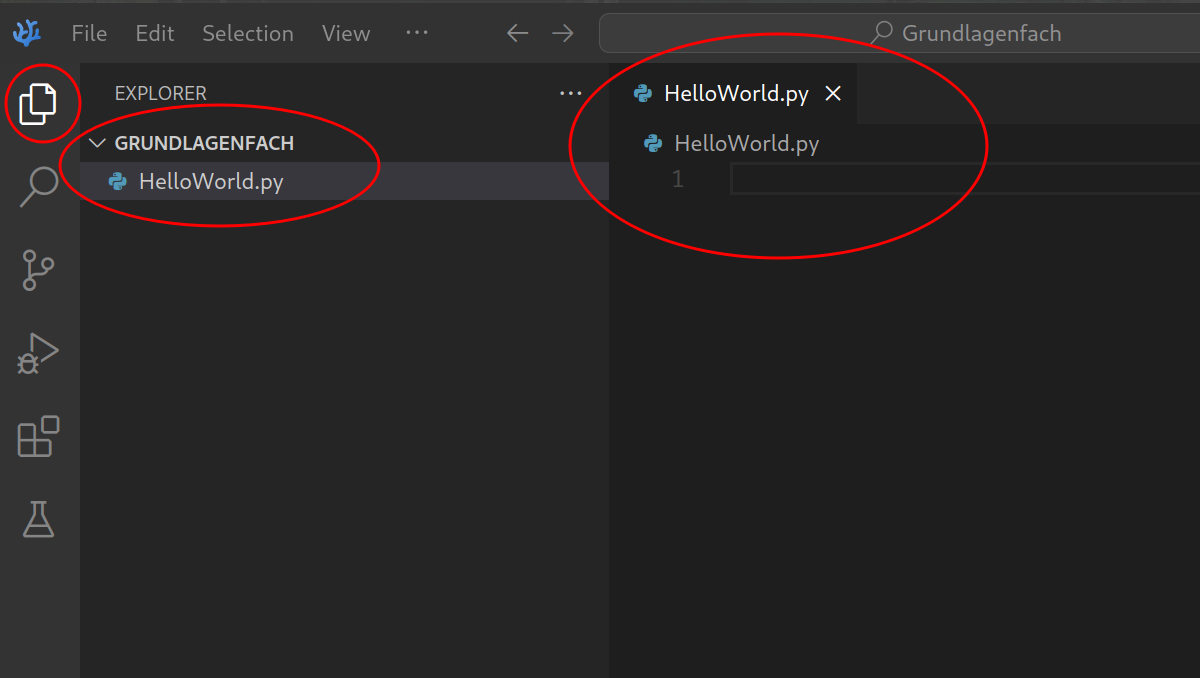
\includegraphics[width=0.9\textwidth]{GrundlagenInfo/00_Programmieren/Skript/Figures/createHelloWorld.png}
	\caption{Python-Programm \texttt{HelloWorld.py} in VSCodium erstellen.}
	\label{fig:createHelloWorld}
\end{figure}

\section{Erstes Python-Programm schreiben und ausführen}
Jetzt schreiben wir unser erstes Python-Programm! Dieses besteht aus nur einer einzigen Zeile und lautet:

\lstinputlisting[language=Python,caption=\texttt{HelloWorld.py},label=listing:helloworld]{GrundlagenInfo/00_Programmieren/Skript/Code/K00_GettingStarted/HelloWorld.py}

Die kleine Ziffer \texttt{1} ist die Zeilennummer (diese wird vom Code-Editor automatisch gesetzt). Wir führen nun das Programm aus (\enquote{lassen das Programm laufen}), indem wir (oben rechts) auf den \emoji{play-button}-Knopf klicken. Bei uns sieht die Situation aus wie in \cref{fig:runHelloWorld}.
\begin{figure}[H]
	\centering
	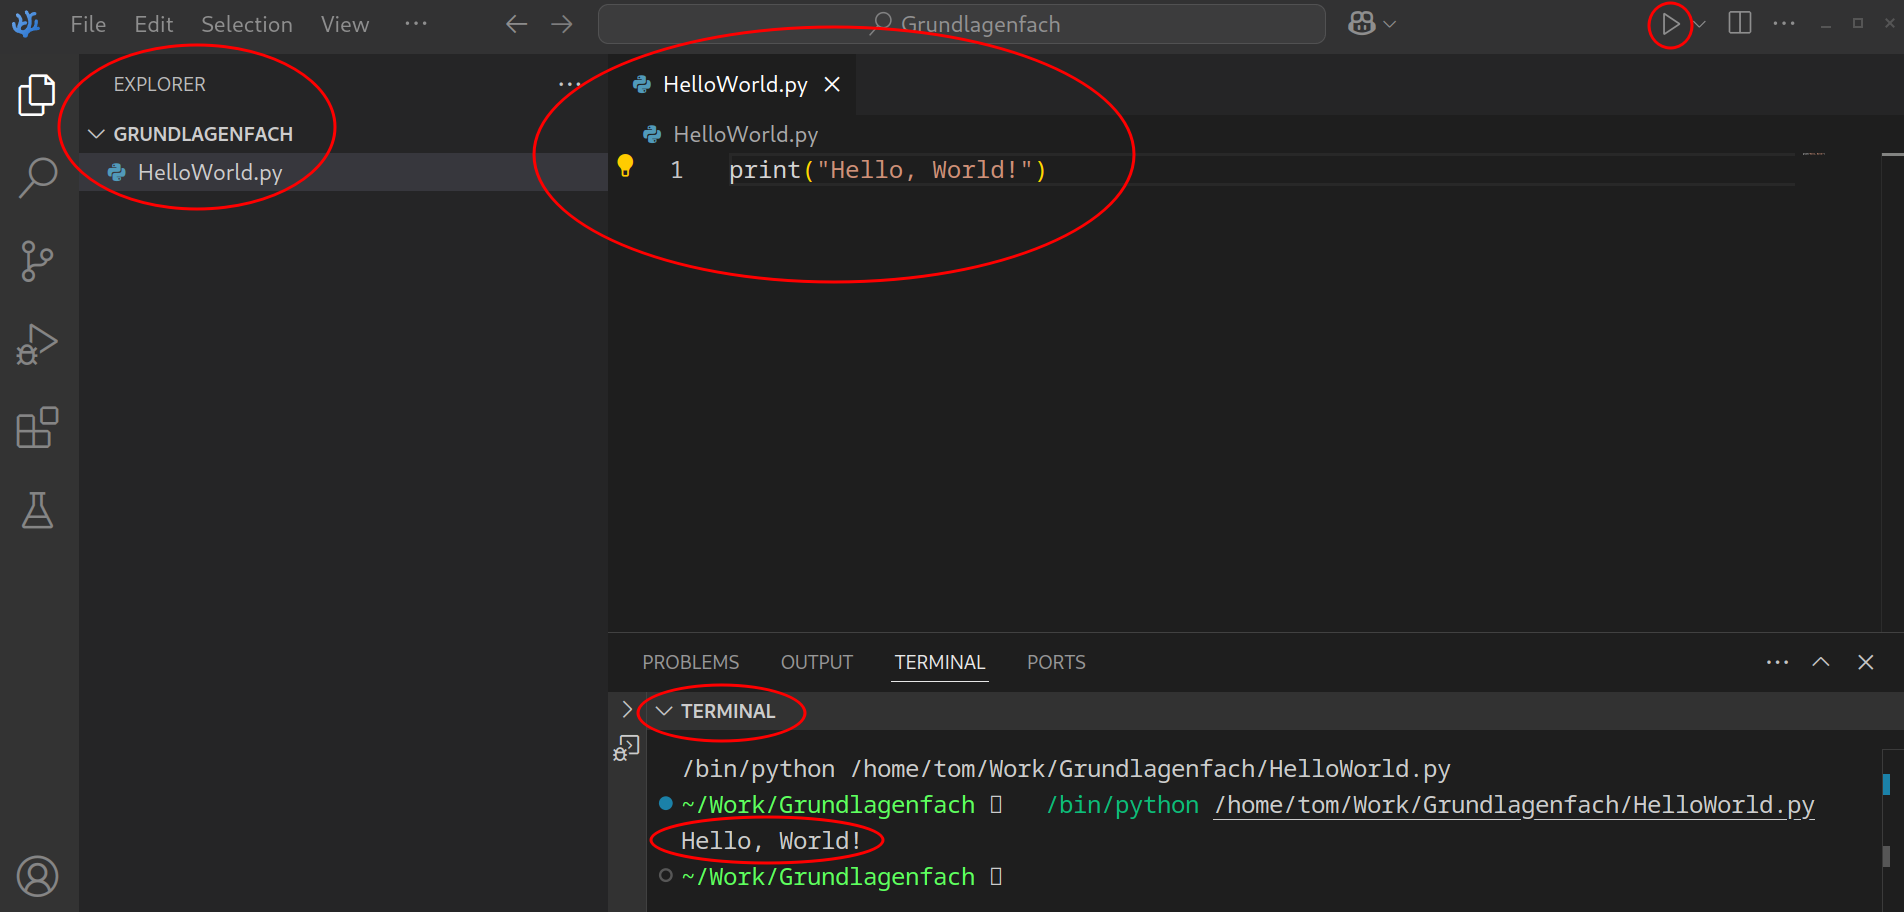
\includegraphics[width=0.9\textwidth]{GrundlagenInfo/00_Programmieren/Skript/Figures/runHelloWorld.png}
	\caption{Python-Programm \texttt{HelloWorld.py} in VSCodium ausführen.}
	\label{fig:runHelloWorld}
\end{figure}
\cref{listing:helloworld}, macht nichts weiter, als den Text
\begin{center}
	\texttt{Hello, World!}
\end{center}
auf der Konsole (en. \textit{terminal}), also im unteren Fenster, auszugeben\footnote{\url{https://de.wikipedia.org/wiki/Hallo-Welt-Programm}}.
